\section{Image-based rendering}

\begin{figure}[htbp]
\centerline{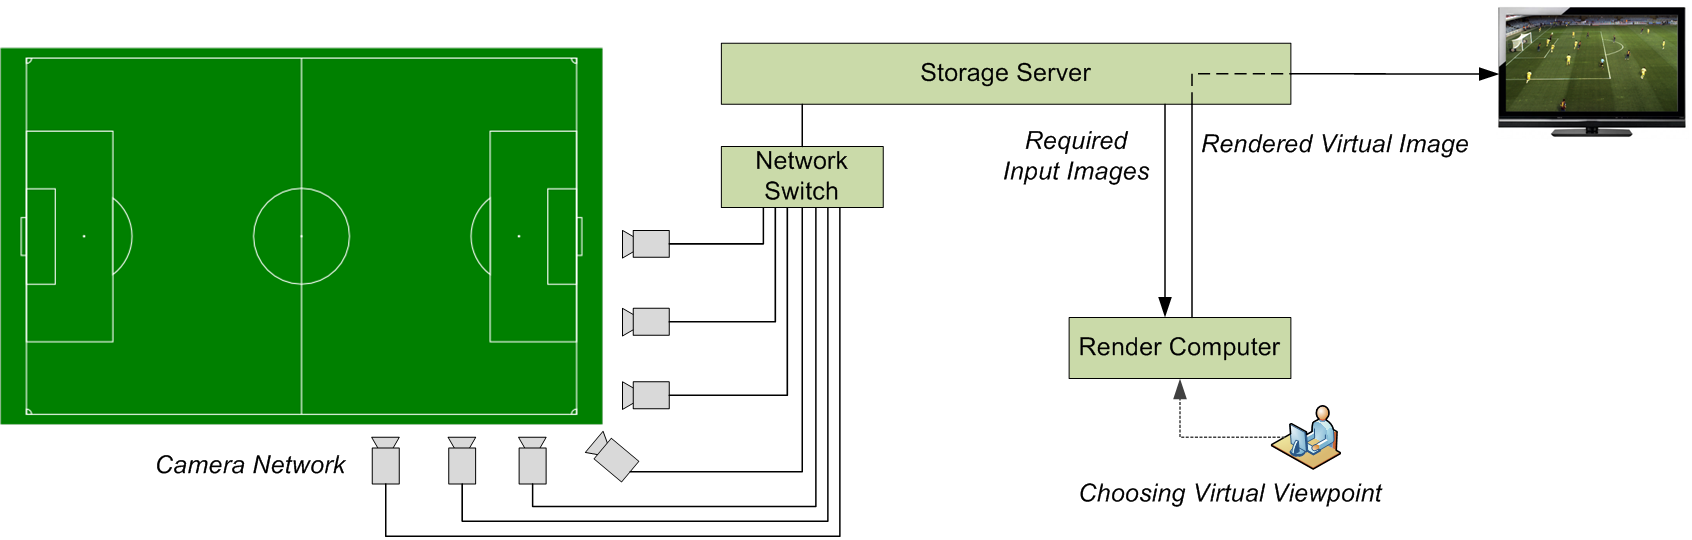
\includegraphics[scale=0.078]{plane_sweeping.png}}
\caption{Overview of the free-viewpoint system. [TODO: cite 02.1]}
\label{fig:plane_sweeping}
\end{figure}

In this section we present a different approach to FVV.
Instead of performing 3D reconstruction, image-based methods generate directly the image of the novel viewpoint.
When multiple cameras are present, plane sweeping can be used [05:Yang et al., 2004] for both small and wide 
baseline setups.
Plane sweeping has already been used for novel view point in soccer scenes. Goorts et al. [05:Goorts
et al., 2012a; Goorts et al., 2013a] present a method
with two plane sweeps and a depth filtering step suitable for smaller baseline 
setups of about 1 meter. 
Moreover, this method has some problems like disappearing players
if they overlap in the image.

